% vim:ts=4:sw=4
% Copyright (c) 2014 Casper Ti. Vector
% Public domain.

\chapter{研究背景}\label{chap:preliminary}
% 中文测试文字。
本章将文中所需要涉及的必要知识进行梳理和阐述,相关概念的定义和简介,不涉及具体证明过程。

\section{PUF工作原理}%
\subsection{工艺涨落}%
集成电路芯片制作可分为设计——流片——验证三大环节。
其中设计者输出给流片厂商的是版图信息。版图则对应着制程中每一层掩膜版的图形,具体到晶体管设计上,版图包括了晶体管宽长比,掺杂区域,互联方式等信息,结合工艺常数,决定了晶体管的设计属性。
在实际流片中,图形转移过程存在套刻精度、刻蚀精度,以及掺杂过程中的退火控制精度等问题。这些操作在实际中存在不可避免的随机误差和系统误差。系统误差在晶圆片上表现为 TT, FF, SS, SF 等不同片区,而随机误差则使得每一颗芯片的时序特征不同,也就是每一个晶体管的表征阈值电压均不相同。
从根本上来说,由于测量系统的局限性,永远不可能复制原子的所有信息,也即不可能使制作后晶体管数值与设计值完全相同。故而误差的累积则造成了工艺涨落,即流片后的晶体管属性与设计属性存在偏差,且在统计学上偏差满足一定的分布规律,下一节将详细说明如何利用由工艺涨落带来的不匹配。
\subsection{信息转换}
由于无法控制工艺涨落的具体数值,也无法预测涨落的大小,因此``芯片制作''这个物理过程符合PUF所要求的``可测不可知''的物理系统,接下来阐述如何给出工艺涨落的观测点。

\begin{figure}[htb!]
\centering
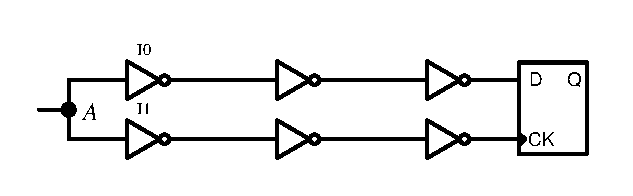
\includegraphics[width=.8\linewidth]{delay-puf}
\caption{延迟-仲裁型 PUF}
\label{fig:delay-puf}
\end{figure}
 
 \begin{figure}[htb!]
 \centering
 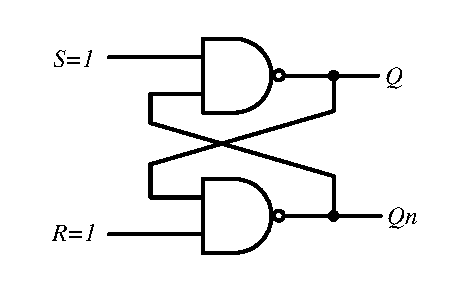
\includegraphics[width=.5\linewidth]{latch-puf}
 \caption{锁存式 PUF}
 \label{fig:latch-puf}
 \end{figure}

PUF将电路工艺参数涨落转换为可输出的电压或电流信号。如图\ref{fig:delay-puf}所示,其中每个反相器和相邻反相器之间的布线在设计上是全等的,但工艺涨落使得反相器中晶体管导电能力必有差异,那么反相器 $ I_0 $ 的信号延迟 $ \Delta t_0 $ 和 $ I_1 $ 的信号延迟 $ \Delta t_1 $ 定满足关系 $ \Delta t_0-\Delta t_1\neq 0 $ ,当输入一个上升沿信号 $ u(t) $ 后, A-D, A-CK  的延迟分别是 $ T_0,T_1 $ ,仲裁器负责判断 D 节点和 CK 节点信号跳变的先后,一个典型的D触发器即可满足仲裁功能。若 D 点信号先于 CK 点上跳,则仲裁器输出逻辑``1'',反之则输出逻辑``0''。由于在得到输出之前并不知道每个反相器的实际延迟,所以不能预测仲裁器的输出,而且每一块相同设计芯片之间的输出也因涨落分布的不同而有差异,因此这样的电路逻辑完成了从工艺涨落到电平信号的信息转换。

又如图\ref{fig:latch-puf}所示,两个反相器及布线在设计上是全等的,上电初始电路处于亚稳态,由于实际的反相器存在偏差,导致其中一个节点的充电电流稍大于另一个节点,使得电路大概率由亚稳态向其中一个稳态过度,此大概率得到的稳态也是工艺涨落的体现,这样的电路也完成了从工艺涨落到存储逻辑值的信息转换。值得注意的是,这里使用了``大概率''的说法,是因为在由亚稳态到稳态的弛豫时间中,存在噪声干扰,从而导致电路向工艺无关的方向变化,这是 PUF 设计中不愿看到的事情。有关 PUF 稳定性的问题,参见\ref{subsec:metrics}节。

\subsection{Weak PUF和Strong PUF}\label{subsec:weakpuf}
类似于\ref{fig:delay-puf}和图\ref{fig:latch-puf}中的电路,利用物理过程的不可控和不可预测性,表达一位或多位稳定信号的系统被称为物理不可克隆函数( Physically Unclonable Function ),其不一定局限于硅基电路,事实上, PUF 概念的首次提出是在光学系统上实现的\supercite{pappu2002physical}。

如果将图\ref{fig:latch-puf}中的结构排成阵列,加上行列选择和译码电路,则构成了类似 SRAM 的阵列,通过不同的``地址''信号可以输出不同的单元信息,像这样的``地址信号''在 PUF 中被称为激励( Challenge ),输出信号被称为响应( Response )。每一个响应都由一个激励相对应,将它们合称为激励-响应对( C-R Pair, CRP )。

\textbf{定义:}若一个 PUF 的激励响应对很少,则称其为 Weak PUF;反之,激励响应对数量级非常多的则称为 Strong PUF\supercite{ruhrmair2014pufs}。

Weak PUF CRP比较单一,没有对外的 IO 接口,以防被穷举,直接将生成的信号送入后续逻辑,实现方式有 SRAM PUF, SA PUF, Latch PUF 等等\supercite{schrijen2012comparative,koeberl2012practical,xiao2014bit,maes2014countering,bhargava2013high}, Weak PUF 多应用于随机数生成、密钥存储方面;

Strong PUF CRP空间非常大,存在对外的 IO 接口,允许通过输入不同的激励得到一组响应,而 CRP 集合的元素量级决定了不可能穷举完所有的 CRP。实现方式有 Arbiter PUF, RO PUF 等等,可实现多种协议。

可以看出 Weak PUF 和 Strong PUF 只是人为地划分,没有明确界限,相较而言,目前以 Strong PUF 的研究和应用居多\supercite{rostami2014quo}。

\subsection{评价指标}\label{subsec:metrics}
PUF (这里特指 Strong PUF,后同)可以用以下几个特定指标衡量:
\begin{itemize}
\item 随机性——对任何一个 CRP 集合的子集,响应(简称 R,后略)的分布应尽可能满足平均分布;
\item 独特性——对任何一个特定的激励(简称 C,后略),一组 PUF 的响应的分布应尽可能满足平均分布;
\item 可靠性——对同样的激励在不同环境温度、电源电压下重复操作应给出相同或大概率相同的响应;
\item 安全性——应对各种已知攻击,详见下一节。
\end{itemize}

除此之外,还有电路通用的面积、功耗、速度等指标,也有用NIST,熵等统计工具代替上述公式\supercite{van2013bias,koeberl2014entropy},特定指标优先级高于通用指标。

下面给出1-3指标的数学定义:

设激励 C 集合$ {c_i} $,响应 R 集合$ {r_i} $,$ r_i=f(c_i) $,若$ R={0,1} $,则随机性可以表征为:
\begin{equation}\label{eq:metric-rand}
Rand=\frac{1}{N}\cdot\sum^{N}f(c_i)
\end{equation}
$ N $ 为 CRP 测试集元素总数,随机性期望值为$ 0.5 $,表明响应应在随机选取的激励下呈平均分布;

独特性表征为:
\begin{equation}\label{eq:metric-uniq}
Uniq=\dfrac{2}{M(M-1)}\sum_{i=1}^{M}\sum_{j=i+1}^{M}\frac{HD(P_i,P_j)}{N}
\end{equation}
\begin{equation}\label{eq:metric-uniq2}
P_i=<f_i(c_0),f_i(c_1),...,f_i(c_n)>
\end{equation}
其中 $ M $ 为测试 PUF 设备总数, $ N $ 为测试激励总数, $ P_i $ 为第 i 个设备 N 个激励响应组成的向量, $ HD(P_i,P_j) $ 指 $ P_i,P_j $ 之间的汉明距离。
独特性期望值为$ 0.5 $,表明任意激励的响应在不同设备间应呈平均分布;

可靠性表征为:
\begin{equation}\label{eq:reliability}
Reliability=\dfrac{1}{MN}\sum_{j}^{M}\sum_{i}^{N}|f(c')-f^{(j)}(c_i)|
\end{equation}
其中N为测试激励总数, $ M $ 为测试重复次数, $ c’ $ 为参考激励,保持不变。可靠性期望值为0。


\section{PUF安全性问题}\label{sec:puf_security}

\subsection{物理模型}
虽然不能精确模拟流片时的掺杂、退火等行为,但是还是可以从宏观上表征一个 PUF 的行为,成这种方式为建模。通常可以将门级电路的驱动能力、延时等抽象为一个平均值W,将R视为C和W的映射 $ R=f(C,W) $。同时,一个好的物理模型有助于快速且准确的仿真验证。

\subsection{参数拟合}
由于 Strong PUF 开放IO端口的特点,若根据攻击者已掌握的一组 CRP 子集,根据建模特点,用机器学习算法拟合出抽象参数$ W $,便可将$ C,W $带入模型中得到 CRP 全集,根据预测率的高低可确定模型建立是否准确抽象了 PUF 的特点。严格来讲,如果一类 PUF 可以被准确抽象出模型,则称该 PUF 是不安全的。但考虑到不是所有模型都能在有限时间内拟合出参数,所以一般认为在特定场合可接受的时间内不能被拟合出参数的 PUF 是安全的。

\section{机器学习算法简介}

\subsection{支持向量机}
支持向量机(Support Vector Machine,SVM),是一种经典的模式识别算法,是 Bell 实验室的 Corinna Cortes 和 Vladimir Vapnik 于1995年首先提出的算法,后经改进,广泛应用于非线性函数拟合,模式识别等机器学习应用中\supercite{cortes1995support}。

SVM 的基本思想是将输入数据映射到一个n维空间中,找到n维空间中的一个超平面能将测试数据集划分开,则该平面将整个空间划分为二,对应着两类不同的数据(如图所示)。

\begin{figure}[h]
\centering
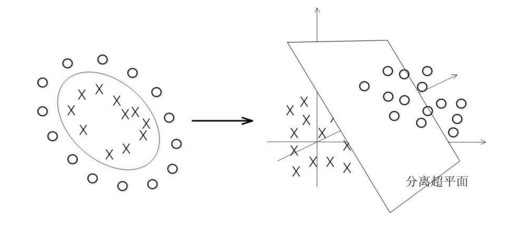
\includegraphics[width=\linewidth]{svm_teach.jpg}
\caption{SVM 映射示意图}
\label{fig:svm_proj}
\end{figure}

下面我们给出线性 SVM 的描述。考虑在n维空间中存在m个特征向量 $ x_1,x_2,x_3,…,x_m $,每个向量具有一个标签( label )``0''或者``1'',期望找到一个超平面( Hyperplane )
\begin{equation}
g(x)=w'x+b=0
\end{equation}
其中 $ w $ 和 $ b $ 是超平面的系数向量。$ g(x) $可以将特征向量分为两类,使得标签``1''向量都满足 $ g(x_i )>0 $,而标签``0''向量都满足 $ g(x_i )<0 $。定义:
\begin{equation}
\gamma=\frac{g(x)}{||w||}
\end{equation}
为向量x到超平面$ g(x)=0 $的几何距离,其中
$ ||w||=\sqrt{w_1^2+w_2^2+...+w_n^2} $
是系数向量w的范数。
为了增加分类的可信度,我们需要找到一个超平面,使得所有特征向量到该超平面的几何距离最大。

事实上并不是所有的数据都是线性可分的,即不存在一个超平面可以将数据集按标签分开。因此非线性 SVM 的做法通常是:
将数据由n维空间映射到$ n+k $维,使得在$ n+k $为空间中数据线性可分。

\subsection{SVM与PUF建模攻击}
如果 PUF 的模型是 $ r=f(c)=sgn(\omega'c+b) $ 的形式,其中 r 是响应,c 是激励,$ \omega $ 是 PUF 内在属性,$ sgn() $是一个符号函数。可以看出 $ g(c)=\omega'c+b=0 $ 便类似于 SVM 中的超平面,在 c 所在空间中,$ g(c) $将向量 c 按标签 r 分为了两类。通过 SVM 找到使 $ \gamma=\frac{g(c)}{||\omega||} $最大的$ \omega $,以使模型达到最大可信度。 SVM 的求解过程在 Matlab 中以 SMO 算法封装实现,而且求解过程并不是本文的关注点,所以不在这里赘述。


\section{相关工作}\label{sec:relatedwork}
\subsection{仲裁型PUF}\label{subsec:apufmodel}
图\ref{fig:delay-puf}展示了一个简单的仲裁型 PUF,图\ref{fig:arb-puf}是一个完整的仲裁型 PUF。其中激励 $ c_i $ 控制双口交换器使得:
\begin{eqnarray}
O_0=c_i?I_1:I_0\\
O_1=c_i?I_0:I_1
\end{eqnarray}
$ O_0,O_1 $ 是交换器的输出, $ I_0,I_1 $ 是输入。这样不同的激励选定了不同的两条数据通路做延迟对比,使得 CRP 空间有 $ 2^n $ 个元素,n为级数。

\begin{figure}[htb!]
\centering
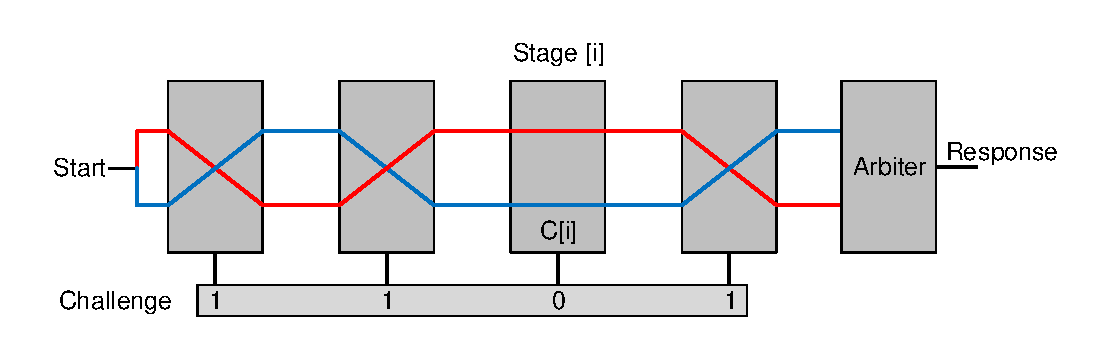
\includegraphics[width=\linewidth]{arbiter_puf}
\caption{仲裁型PUF}
\label{fig:arb-puf}
\end{figure}

将每一个交换器抽象为4条通路,设每条通路延迟分别为 $ p_i,q_i,r_i,s_i $ (如图\ref{fig: switcher}所示),信号到达输入的时间分别为 $ t_1(i),t_2(i) $,输出的时间分别为 $ t_1(i+1),t_2(i+1) $,则有:
\begin{eqnarray}\label{eq:apuf-cell}
t_1(i+1)=c_i?t_2(i)+r_i:t_1(i)+p_i \\
t_2(i+1)=c_i?t_1(i)+q_i:t_2(i)+s_i
\end{eqnarray}

\begin{figure}[htb!]
\centering
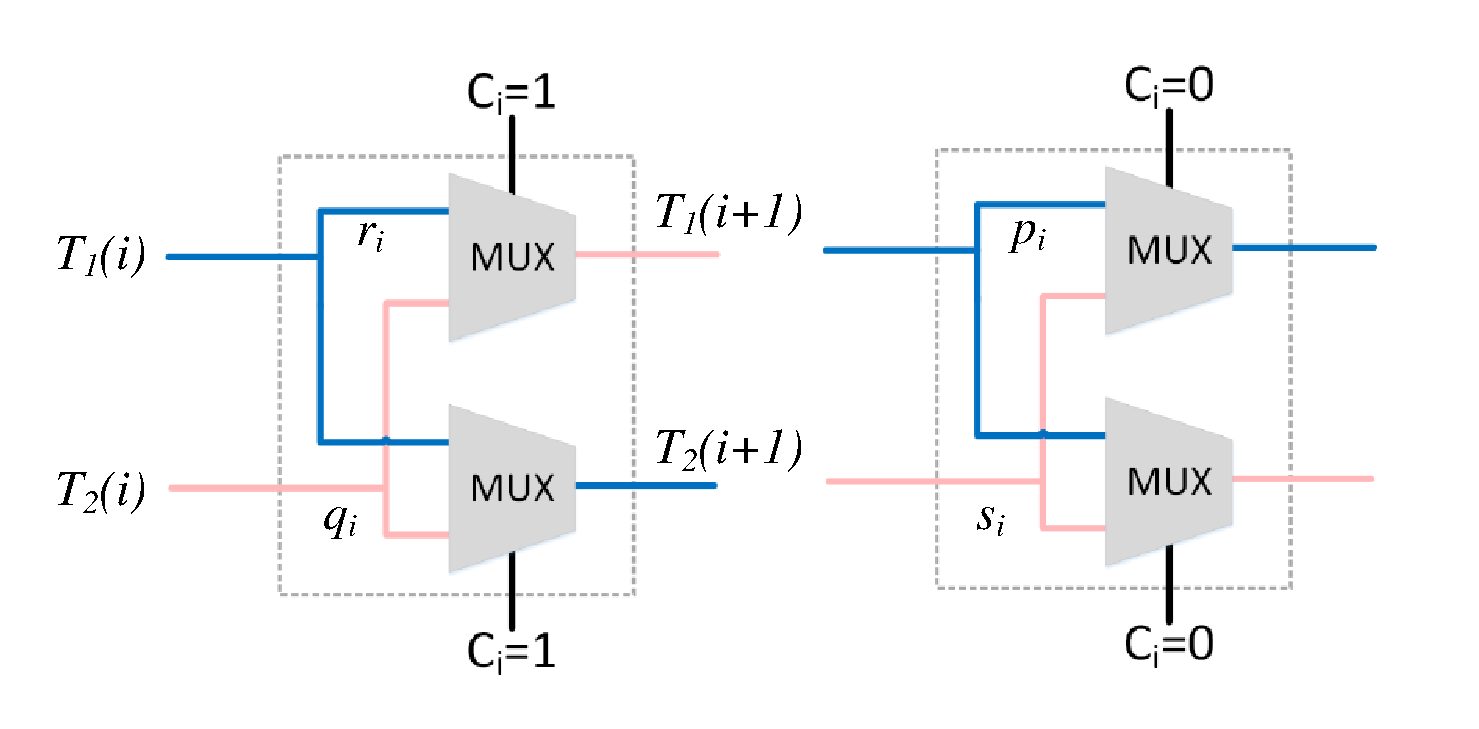
\includegraphics[width=\linewidth]{switcher}
\caption{双口交换器模型}
\label{fig: switcher}
\end{figure}

为了方便数学推导,将逻辑``0''记为-1,将逻辑``1''记为+1,则``异或''等价``乘''运算,故\ref{eq:apuf-cell}可化为
\begin{eqnarray}
t_1(i+1)=\frac{1+c_i}{2}(t_2(i)+r_i)+\frac{1-c_i}{2}(t_1(i)+p_i) \\
t_2(i+1)=\frac{1+c_i}{2}(t_1(i)+q_i)+\frac{1-c_i}{2}(t_2(i)+s_i)
\end{eqnarray}
两式做差得:
\begin{equation}
\delta (i+1)=t_1(i+1)-t_2(i+1)=-c_i\delta(i)+\frac{r_i-q_i+p_i-s_i}{2}+\frac{c_1}{2}(r_i-q_i-p_i+s_i)
\end{equation}
求解此递推关系式最终可得:
\begin{equation}
\delta(n)=p'd
\end{equation}
其中向量 $ p=<p_0,p_1,…,p_n> $, $ p_i=\Pi_{k=i+1}^{n}c_k $,向量 $ d=<\alpha_1,\alpha_2+\beta_1,…,\alpha_n+\beta_(n-1),\beta_n> $, $ \alpha_i=\frac{r_i-q_i-p_i+s_i}{2},\beta_i=\frac{r_i-q_i+p_i-s_i}{2} $,并定义 $ p_n $ 为常数1。由于 $ r=f(c)=sgn[\delta(n)] $,所以存在n维空间上的超平面 $ p'd=0 $ 将特征向量p按r标签分开。在这里p是向量c在同维空间中的一个映射,而向量d代表了每个交换器的延迟时间,是 PUF 的本征属性。

通过一组已知的 CRP 子集,我们可以确定一组向量d,用 SVM 算法找到具有最大可信度的d向量,作为延迟时间的估值,这样便推导出了仲裁型 PUF 的模型,对于未知响应的激励 $ c’ $,根据 $ sgn(p'd) $ 可预测其响应。根据文献\parencite{lim2005extracting}的数据,当训练集大小超过2000时,预测准确率在95\%以上。

\subsection{仲裁型PUF的改进}
因为仲裁型 PUF 的观测点——延迟时间的累加是线性过程,所以容易建立适合 SVM 算法的模型。在文献\parencite{lim2005extracting}中作者提出了改进方案——前馈仲裁型 PUF (如图\ref{fig: ffpuf}),用中间值 $ sgn[\delta(k)] $ 作为交换器的控制信号,如果用同样的思路建立模型,那么在模型表达式中存在非线性函数$ sgn $,不能再直接使用 SVM 算法求解代表延迟的d向量。

\begin{figure}[htb!]
\centering
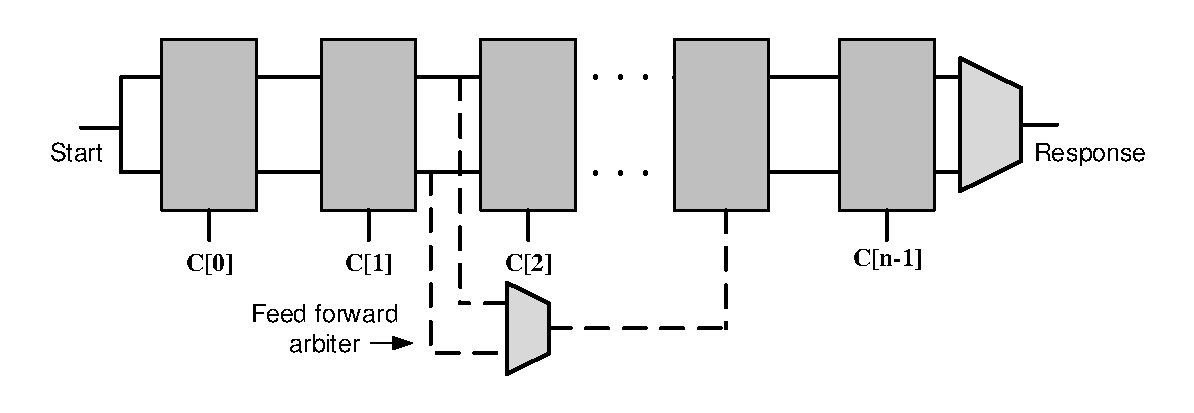
\includegraphics[width=\linewidth]{feedforwardpuf}
\caption{前馈仲裁型 PUF}
\label{fig: ffpuf}
\end{figure}

但\parencite{lim2005extracting}中同样提到了 FFPUF 的攻击方法,而且可以在有限时间内完成,说明这种方法或单独使用这种方法仍是不安全的。

\subsection{异或输出的PUF}\label{subsec:xormethod}

\parencite{suh2007physical}中, G. Edward Suh 和 S. Devadas 提出了 XOR PUF,即是将采用多个传统仲裁型 PUF,给予相同的激励,并且将响应值全部异或起来。异或运算具有非线性特性,具体来讲,两个同激励的 PUF 异或之后输出可以表达成:
\begin{equation}\label{eq:xor-model}
R=p'd\times p'e
\end{equation}
d, e 分别代表两个 PUF 的内在参数,若要使R线性可分,必须要写成 $ P’D $ 的形式,将式\ref{eq:xor-model}展开可以写成 $ P’D $ 的形式,但在这里$ D $是 $ \frac{n(n-1)}{2} $ 维的向量, SVM 的计算复杂度由n上升到了 $ n^2 $,经过多个 PUF 异或后可以将运算复杂度上升到不能在有限时间尺度上求解。

异或的非线性特性不依赖于具体的 PUF 形式,因此是一种通用的增加 PUF 安全性的做法。但是异或的缺点显而易见:面积资源开销增加了N倍,同时误码率也增加了。

\subsection{双稳态环路PUF}
2011年Qingqing Chen等人在会议 Hardware-Oriented Security Transaction 上提出了一种新的PUF,双稳态环路型 PUF(Bistable Ring PUF,如图\ref{fig: brpuf})。  BRPUF 采用了偶数级反相器级联构成回路具有双稳态的特性构建 PUF 的观测点,具有新颖性,并且作者声称其环路具有非线性结构,较传统仲裁型 PUF 安全性更高\supercite{chen2011bistable}。

截止本文撰写时,仅有 Qingqing Chen 本人在文献\parencite{chen2012characterization}中对 BRPUF 做了特性分析; D. Schuster 和 R. Hesselbarth 对 BRPUF 用单层神经网络进行建模\supercite{schuster2014evaluation}。

\begin{figure}[htb!]
\centering
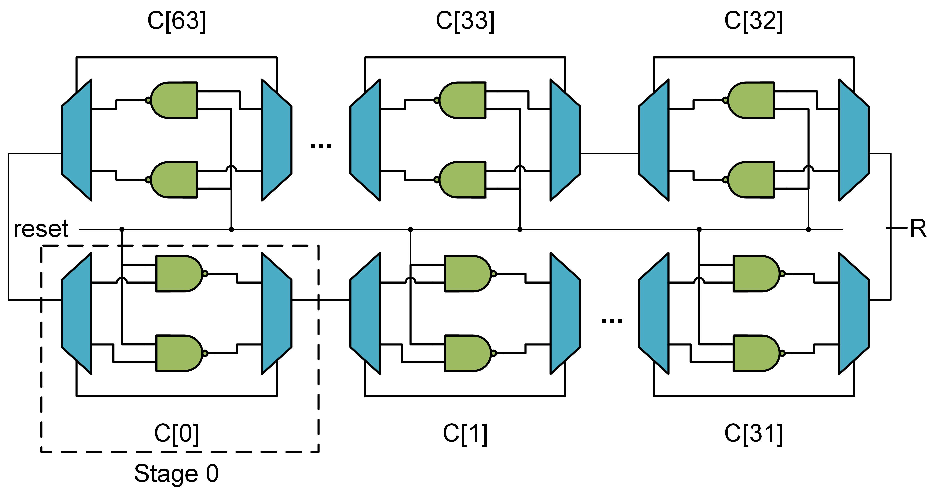
\includegraphics[width=\linewidth]{BRPUF}
\caption{双稳态环路型PUF}
\label{fig: brpuf}
\end{figure}

\section{本章小结}
本章介绍了 PUF 工作机制, PUF 的评价标准;介绍了针对 PUF 的机器学习建模攻击算法;以及列举了近期相关研究者的工作。 PUF 适合生成片间无关的大量激励-响应数据对,且占用资源和功耗相较于传统电路非常小,适合于物联网移动端芯片的内嵌安全模块。
但是目前 PUF 面临建模攻击的威胁,强大的机器学习算法可以用很小的代价推算出 PUF 的所有信息,这样致使一般的 PUF 原型设计不能直接应用于工程芯片。大量的研究者给出了新的设计方案,在下一章中,本文将对其中一个设计进行分析,并提出 PUF 设计的指导性标准。
